
\chapter{}\label{ch:auf1}
In dieser Aufgabe wird der bürstenlose Gleichstrommotor (BLDC) mit der Spannung $ U_{AP} $ und dem Strom $ I_{AP} $ betrieben. Der BLDC ist starr über eine Welle mit dem Gleichstrommotor (GM) verbunden. Der GM dient hierbei als Last für den BLDC. Der GM fungiert als Generator und wird durch den Antrieb des BLDC in Bewegung versetzt und erzeugt somit eine Spannung $ U_{AL} $, welche dann einen Strom $ I_{AL} $ verursacht. Wir wollen diesen Strom $ I_{AL} $ messen. Zu beachten ist, dass $ U_{AL} $ nur Werte im Bereich [0V bis 24V] annehmen kann. \\Vom Hersteller sind für die Belastungsmaschine folgende Daten gegeben:
\begin{center}
	$ R_{AL} = 0,4\Omega $ \hspace{2cm} $ C_{E}\Psi_{PML} = 0,4Vs $\\ 
\end{center}

\section{}\label{sec:1a}
\textit{Skizzieren Sie die Leerlaufspannung der Belastungsmaschine in Abhängigkeit von der Drehzahl $ N_{P} $ des bürstenlosen Gleichstrommotors im Bereich 0-3000 $ min^{-1} $.}\\
Zur Ermittlung der Kennlinie ziehen wir folgende Formel heran:
\begin{equation}
	U_{i} = C_{E}\Psi~N
	\label{eq:1a:Ui}
\end{equation}
Die Drehzahl wird von $ min^{-1} $ auf $ s^{-1} $ umgerechnet ($ 3000 min^{-1} = 50 s^{-1} $). Wir setzen nun die beiden Drehzahlen in die Formel \ref{eq:1a:Ui} ein. Einmal berechnen wir den Wert, wenn der Motor stillsteht (0 Umdrehungen pro Sekunde), sowie ein weiteres Mal, wenn der Motor 50 Umdrehungen pro Sekunde macht, (also der maximal geforderten Drehzahl). Da wir in den Berechnungen der beiden Werte nur N ändern ist die Änderung des Ergebnisses proportional, also direkt abhängig von der eingesetzten Drehzahl. Dies bedeutet es handelt sich bei dem in Abbildung \ref{fig:1a:leerlauf} zu skizzierenden Graphen um eine Gerade. 
\begin{table}[h]
	\centering
	\begin{tabular}{p{1.25cm} | p{1.25cm}}
		$ N $ & $ U_{i} $\\ \hline &\\[-1em]
		0 & 0 \\
		$ 50s^{-1} $ & $ 20V $
	\end{tabular}
\end{table}

\begin{figure}[h]
	\centering
	% This file was created by matlab2tikz.
%
%The latest updates can be retrieved from
%  http://www.mathworks.com/matlabcentral/fileexchange/22022-matlab2tikz-matlab2tikz
%where you can also make suggestions and rate matlab2tikz.
%
\definecolor{mycolor1}{rgb}{0.00000,0.44700,0.74100}%
%
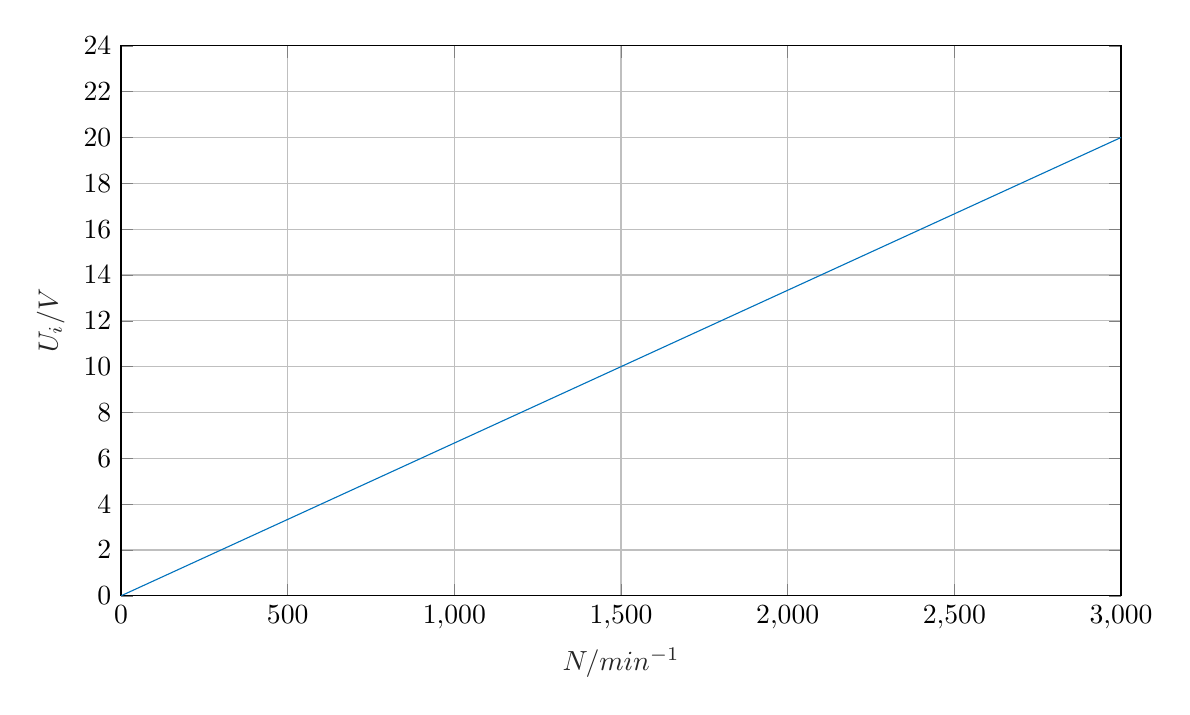
\begin{tikzpicture}

\begin{axis}[%
width=5in,
height=2.75in,
at={(0.758in,0.481in)},
scale only axis,
xmin=0,
xmax=3000,
xtick={   0,  500, 1000, 1500, 2000, 2500, 3000},
xlabel style={font=\color{white!15!black}},
xlabel={$ N / min^{-1} $},
ymin=0,
ymax=24,
ytick={ 0,  2,  4,  6,  8, 10, 12, 14, 16, 18, 20, 22, 24},
ylabel style={font=\color{white!15!black}},
ylabel={$ U_{i} / V $},
axis background/.style={fill=white},
xmajorgrids,
ymajorgrids
]
\addplot [color=mycolor1, forget plot]
  table[row sep=crcr]{%
0	0\\
3000	20\\
};
\end{axis}
\end{tikzpicture}%
	\caption{Leerlaufspannung der Belastungsmaschine}
	\label{fig:1a:leerlauf}
\end{figure}



\section{}\label{sec:1b}
\textit{Für die Belastung des BLDC wird an die Ankerklemmen des konventionellen Gleichstrommotors anstelle einer Spannungsquelle ein veränderlicher Widerstand $ R_{L} $ angeschlossen. Welchen Wert muss dieser Widerstand haben, um bei einer Drehzahl von $ N_{P} = 2000 min^{-1} $ des BLDC ein Lastmoment von $ M_{L} = 0,25Nm $ zu erzeugen?}\\ Zur Ermittlung des Wertes des Widerstands ziehen wir folgende Formel zur Bestimmung des Lastmomentes heran
\begin{equation}
	M_{L} = C_{M}\Psi_{PML}I_{A}
	\label{eq:1b:ML}
\end{equation}
Da der BLDC starr gekoppelt ist mit dem GM gilt: Lastmoment ($ M_{L} $) = Inneres Motormoment ($ M_{Mi} $). Aufgrund dieser Erkenntnis gilt:
\begin{equation}
	M_{Mi} = M_{L} = C_{M}\Psi_{PML}I_{A} = C_{M}\Psi_{PML}\frac{U_{i}}{R_{AL}+R_{L}} = \frac{C_{E}}{2\pi}\Psi_{PML}\frac{U_{i}}{R_{AL}+R_{L}}
	\label{eq:1b:MMi}
\end{equation}

Formel \ref{eq:1b:MMi} wird nach $R_{L}$ umgestellt, so ergibt sich folgender Zusammenhang:\\
\begin{equation}
	R_{L} = \frac{C_{E}\Psi_{PML}U_{i}}{2\pi M_{L}} - R_{AL}
\end{equation}
Damit wir $ R_{L} $  bestimmen können, müssen wir zuerst über Formel \ref{eq:1a:Ui} $ U_{i} $ ermitteln. Hierdurch ergibt sich $ R_{L} = 8,07\Omega$. Zum Schluss dieser Berechnung haben wir eine Einheitenprüfung durchgeführt, die erhaltene Einheit soweit plausibel.

\section{}\label{sec:1c}
\textit{Bestimmen Sie den Zusammenhang $ N_{P}(M_{L}) $ für einen fest vorgegebenen Lastwiderstand $ R_{L} $.}\\
Die Gleichung \ref{eq:1a:Ui} aus Aufgabenteil \ref{sec:1a}) wird im Folgenden mit einbezogen. Wir ersetzen $ U_{i} $ durch diese Formel. Daraus ergibt sich für $ R_{L} $ nun folgender Zusammenhang:
\begin{equation}
	R_{L} = \frac{C_{E}\Psi_{PML}C_{E}\Psi_{PML}N_{P}}{2\pi M_{L}} - R_{AL}
	\label{eq:1c:RL}
\end{equation}
Nach entsprechender Umstellung der Formel ergibt sich für $ N_{P} $:
\begin{equation}
	N_{P}(M_{L}) = \frac{2\pi (R_{AL}+R_{L})M_{L}}{C_{E}^{2}\Psi_{PML}^{2}}
	\label{eq:1c:NP}
\end{equation}


\clearpage



